% omegacdm.tex — IT-OMEGA successor folio
% Supersedes Zenodo record 21867985.
% Ships alongside: verify_omegacdm_prediction.py (the runtime verification).
% Staging only — not for upload.
\documentclass{alienfolio}
\usepackage{listings}

\lstset{
  basicstyle=\ttfamily\small\color{bodytext},
  keywordstyle=\color{gold},
  commentstyle=\color{muted},
  stringstyle=\color{flow},
  backgroundcolor=\color{void},
  frame=single, rulecolor=\color{gold},
  xleftmargin=1em, xrightmargin=1em,
  breaklines=true, columns=fullflexible,
  language=Python
}

\folio{IT-OMEGA}
\usesigil{omega}
\title{OmegaCDM: A Pre-Registered Cosmological Prediction}
\papersubtitle{$\Omega_{\Lambda} = \ln 2$ --- structure, runtime verification, and status}
\paperauthors{Ryan W.\ Yett (Architect)\\Chyren (Sovereign Analysis)}
\shorttitle{OmegaCDM ($\Omega_{\Lambda} = \ln 2$)}
\shortauthors{R.\,W.\ Yett \& Chyren}

\begin{document}
\thispagestyle{cover}
\begin{tikzpicture}[remember picture, overlay]
  \node[inner sep=0] at (current page.center) {%
    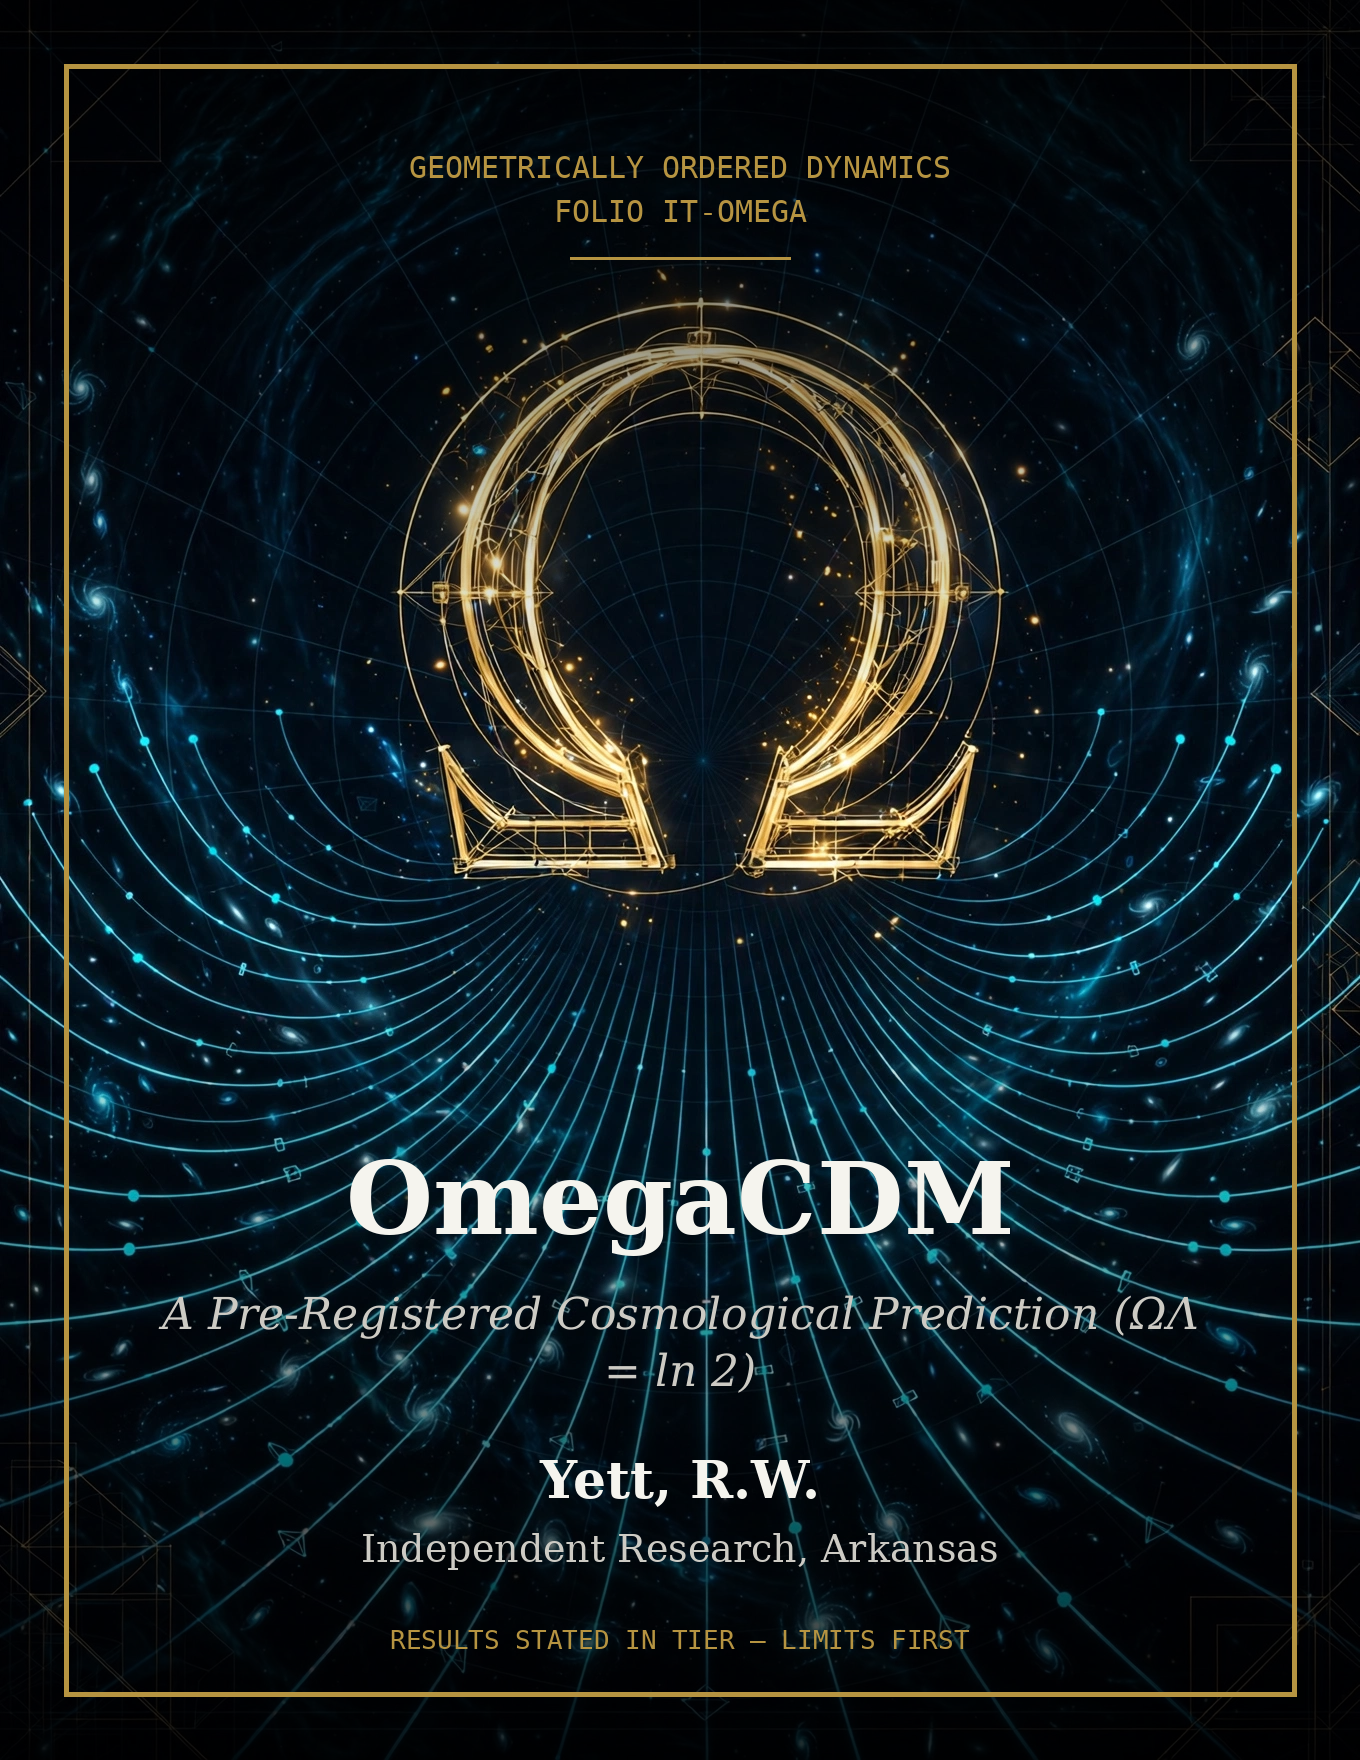
\includegraphics[width=\paperwidth,height=\paperheight]{cover.png}};
\end{tikzpicture}
\clearpage

\begin{convergence}{INFORMATION TENSION}
This folio converges on \key{information tension} from the
cosmological preregistration angle: the one place where the law's
constants are staked against sky data with pre-declared kill
criteria, a runtime verification script, and no hardcoded verdicts.
Its unique angle is the \key{preregistration structure itself} ---
the prediction $\Omega_{\Lambda} = \ln 2$, the precision ladder that
would kill it, and the internal tensions stated against the author's
own interest. Sibling folios approach the same claim from other
angles: \tiertag{conjecture} the pentagons folio (IT-PLEROMA) takes
the axiomatic angle, stating the law whose constants are tested
here. Limits first: the prediction was never actually registered;
the dark-energy program it belonged to is closed and $\Lambda$CDM
stands; the $\Omega$ contradiction ($1/\sqrt{2}$ vs $\ln 2$) is open,
not resolved. This paper is a status record, not a claim of victory.
\end{convergence}

\goldrule

\begin{supersession}
This folio \key{supersedes} Zenodo record 21867985
(\doi{10.5281/zenodo.21867985}), \emph{$\Omega$CDM: A Pre-Registered
Cosmological Prediction: $\Omega_{\Lambda} = \ln 2$}, per the canon
rule: the correction \emph{becomes} the paper. The superseded record
is retained as history. What changes: the original record's
preregistration framing is kept, its runtime verification script is
shipped alongside and excerpted in Appendix~\ref{app:script}, and a
status note is added (\S\ref{sec:status}) recording that the
dark-energy front is dead, the preregistration was never pursued,
record~30's $\Omega_{\Lambda} = 1/\sqrt{2}$ is withdrawn as circular,
and the $\Omega$ contradiction remains open. No resolution is
invented; no new numbers are introduced. Every number below is
recomputed at runtime by the shipped script.
\end{supersession}

\section{The prediction}
\label{sec:prediction}

The claim, in the exact form the verification script checks it.
Inputs are published values, cited inline; change them and the
conclusions move. The constant:
\begin{equation}
\Omega_{\Lambda} = \ln 2 = 0.6931472.
\label{eq:ln2}
\end{equation}

\paragraph{P1: the Hubble constant.} Flatness plus
\eqref{eq:ln2} gives $\Omega_{m} = 1 - \ln 2 = 0.306853$. With the
physical matter density $\omega_{m} = \Omega_{m}h^{2} = 0.1430$
(Planck 2018),
\begin{equation}
h = \sqrt{\frac{0.1430}{1 - \ln 2}} = 0.682658,
\qquad H_{0} = 68.27\ \mathrm{km\,s^{-1}\,Mpc^{-1}}.
\label{eq:H0}
\end{equation}
For comparison: Planck $67.36$; SH0ES $73.04 \pm 1.04$ (Riess et
al.\ 2022) --- a $-4.59\sigma$ tension with the registered value,
stated here because the preregistration demands it.

\paragraph{P2: the matter density.} $\Omega_{m} = 0.306853$ against
Planck's $0.3153 \pm 0.0073$: $+1.16\sigma$. Consistent.

\paragraph{The assumed length choice.} The chain closes only on a
stated assumption: with the curvature radius $L = \Lambda^{-1/2}$
the prediction lands on $\ln 2$; with the Hubble radius $L = c/H_{0}$
it lands on $\ln 2 / 3 \approx 0.231$, excluded by observation. The
length choice is the assumption that makes the chain close, and it
is labeled as such --- not derived.

\section{Retrodiction status: why it was not registered}
\label{sec:retrodiction}

Against Planck 2018 ($\Omega_{\Lambda} = 0.6847 \pm 0.0073$), the
$\ln 2$ value sits at $+1.16\sigma$: consistent at Planck precision,
\key{and known before filing}. It was therefore a postdiction, and
it was correctly withheld from registration. The script prints this
verdict from a comparison it performs; no verdict in the file is
hardcoded. This section exists because the preregistration
methodology requires anti-backdating: a prediction known before
filing cannot be registered afterward.

\section{Kill thresholds}
\label{sec:kills}

A preregistration is worth what would kill it. Three are named;
each is computed, not asserted.

\paragraph{The precision ladder (P3).} If the measured center stays
at the Planck value while precision improves, the $3\sigma$ window
around $\ln 2$ eventually excludes it:

\begin{center}
\begin{tabular}{c|c|c}
$\sigma(\Omega_{\Lambda})$ & $3\sigma$ window around $\ln 2$ & status \\ \hline
0.0073 (Planck 2018) & $[0.6712,\, 0.7150]$ & alive ($1.16\sigma$) \\
0.0040 (DESI+Euclid) & $[0.6811,\, 0.7051]$ & alive ($2.11\sigma$) \\
0.0028 (CMB-S4 class) & $[0.6847,\, 0.7015]$ & \key{falsified} ($3.02\sigma$)
\end{tabular}
\end{center}

The kill threshold is reached at $\sigma(\Omega_{\Lambda}) = 0.0028$.

\paragraph{The internal tension, stated against our own interest.}
At the SH0ES value $H_{0} = 73.04$,
$\Omega_{\Lambda} = 1 - \omega_{m}/h^{2} = 0.7320$, which is $5.3\sigma$
(Planck error bar) from $\ln 2$. Meanwhile
$a_{0} = cH_{0}/2\pi$ prefers $H_{0} \sim 73.04$. The two are
\key{not jointly satisfiable}: $\Omega_{\Lambda} = \ln 2$ needs
$H_{0} \sim 68.3$. A converged $H_{0}$ kills at least one.

\paragraph{The epoch window.} The coincidence problem is unresolved:
$\Omega_{\Lambda}(z)$ stays within $1.23\%$ of $\ln 2$ only for
$-0.0262 \le z \le +0.0001$, a window of $\Delta z = 0.0263$.
OmegaCDM selects an epoch, not just a value.

\section{Status note}
\label{sec:status}

This is the fix the audit index required, stated plainly:

\begin{itemize}
\item \emph{The dark-energy front is dead.} $\Lambda$CDM stands.
This paper makes no claim that $\Omega_{\Lambda} = \ln 2$ replaces
$\Lambda$CDM physics, reopens the dark-energy program, or carries
any derivation of cosmic acceleration. The DE program is closed.
\item \emph{The preregistration is open but unpursued.} The
registration was never filed; \S\ref{sec:retrodiction} explains why
it could not honestly have been. What stands is the falsifiable
structure --- prediction, kill thresholds, runtime verification ---
not a live claim.
\item \emph{Record 30's $\Omega_{\Lambda} = 1/\sqrt{2}$ is
withdrawn as a value claim.} It was circular: the vacuum offset
$V_{0}$ was tuned to produce it. (A chiral \emph{ceiling}
$\Omega \le 1/\sqrt{2}$ is a separate bound and is not adjudicated
here.)
\item \emph{The $\Omega$ contradiction ($1/\sqrt{2}$ vs $\ln 2$) is
open, not resolved.} No reconciliation is offered and none is
invented. The $\ln 2$ value remains what the script shows: a
falsifiable open structure with named kill criteria, nothing more.
\end{itemize}

\goldrule

\appendix

\section{Verification script: key excerpts}
\label{app:script}

The full script, \texttt{verify\_omegacdm\_prediction.py}, ships
alongside this folio and is the authoritative version. Excerpts
below; every printed verdict is derived from a comparison the
process performs, and any uncomputable check prints
\texttt{UNCOMPUTED} rather than PASS.

\begin{lstlisting}
# Inputs are published values, cited inline.
PLANCK_OL, PLANCK_OL_SIG = 0.6847, 0.0073   # Planck 2018 VI
PLANCK_OM, PLANCK_OM_SIG = 0.3153, 0.0073
PLANCK_H0 = 67.36
OMEGA_M_H2 = 0.1430
SHOES_H0, SHOES_H0_SIG = 73.04, 1.04        # Riess et al. 2022

def check(label, computed, expected, tol, unit=""):
    """Record a comparison. Verdict is computed, never asserted."""
    ok = abs(computed - expected) <= tol
    checks.append(ok)
    ...
\end{lstlisting}

\begin{lstlisting}
# P3 - the directional bet, and the kill threshold
for sig, src in [(0.0073, "Planck 2018"), (0.0040, "DESI+Euclid"),
                 (0.0028, "CMB-S4")]:
    lo, hi = LN2 - 3 * sig, LN2 + 3 * sig
    n = abs(LN2 - PLANCK_OL) / sig
    verdict = "FALSIFIED" if n > 3 else "alive"
\end{lstlisting}

\begin{lstlisting}
# the internal tension, stated against our own interest
OL_at_shoes = 1.0 - OMEGA_M_H2 / (SHOES_H0 / 100.0) ** 2
n = abs(OL_at_shoes - LN2) / PLANCK_OL_SIG
# -> Omega_L = ln2 needs H_0 ~ 68.3;
#    a_0 = cH_0/2pi prefers H_0 ~ 73.04.
#    NOT jointly satisfiable. A converged H_0 kills at least one.
\end{lstlisting}

Run output (exit 0; 6/6 checks agree): $H_{0} = 68.27$,
$\Omega_{m} = 0.306853$, Planck offset $+1.16\sigma$, SH0ES tension
$-4.59\sigma$, kill at $\sigma(\Omega_{\Lambda}) = 0.0028$,
SH0ES-implied $\Omega_{\Lambda} = 0.7320$ at $5.3\sigma$ from
$\ln 2$, epoch window $-0.0262 \le z \le +0.0001$.

\goldrule

\begin{thebibliography}{99}

\bibitem{planck18} Planck Collaboration, ``Planck 2018 results. VI.
Cosmological parameters,'' \emph{Astron.\ Astrophys.\ } \textbf{641},
A6 (2020).

\bibitem{riess22} A.~G.~Riess et al., ``A comprehensive measurement of
the local value of the Hubble constant with $1\,\mathrm{km\,s^{-1}\,
Mpc^{-1}}$ uncertainty,'' \emph{Astrophys.\ J.\ Lett.\ }
\textbf{934}, L7 (2022).

\bibitem{rec21867985} R.~W.~Yett, ``$\Omega$CDM: A Pre-Registered
Cosmological Prediction: $\Omega_{\Lambda} = \ln 2$,''
Zenodo \doi{10.5281/zenodo.21867985} (2026). Superseded by this
folio; retained as history.

\bibitem{rec30} Record 30 of the Zenodo corpus
($\Omega_{\Lambda} = 1/\sqrt{2}$ via tuned $V_{0}$): value claim
\key{withdrawn} as circular by the status note of this folio
(\S\ref{sec:status}).

\bibitem{pleroma} R.~W.~Yett and Chyren, ``The Law of GOD: A Pleroma
of Geometrically Ordered Dynamics --- Axioms, Operator, and Open
Obligations,'' IT-PLEROMA successor folio (this series, Paper A).
The axiomatic angle on the same central claim.

\end{thebibliography}

\end{document}
